\documentclass[a4paper]{article}
\usepackage[margin=5mm,top=20mm]{geometry}
\usepackage[utf8]{inputenc}

\usepackage{microtype}

\usepackage{graphicx}

\usepackage{color}

\usepackage{tikz}

\usepackage{pifont}

\usepackage{fourier-orns}

\usepackage{calculator}
% Card Arena v0.1 Colors

% Character colours
\definecolor{red}{RGB}{244,56,36}
\definecolor{blue}{RGB}{36,45,140}
\definecolor{purple}{RGB}{128,0,128}
\definecolor{green}{RGB}{63,165,56}
\definecolor{orange}{RGB}{216,128,43}
\definecolor{teal}{RGB}{51,179,198}
\definecolor{yellow}{RGB}{244,226,66}
\definecolor{brown}{RGB}{145,95,39}


\begin{document}
\begin{center}
\pagestyle{empty}

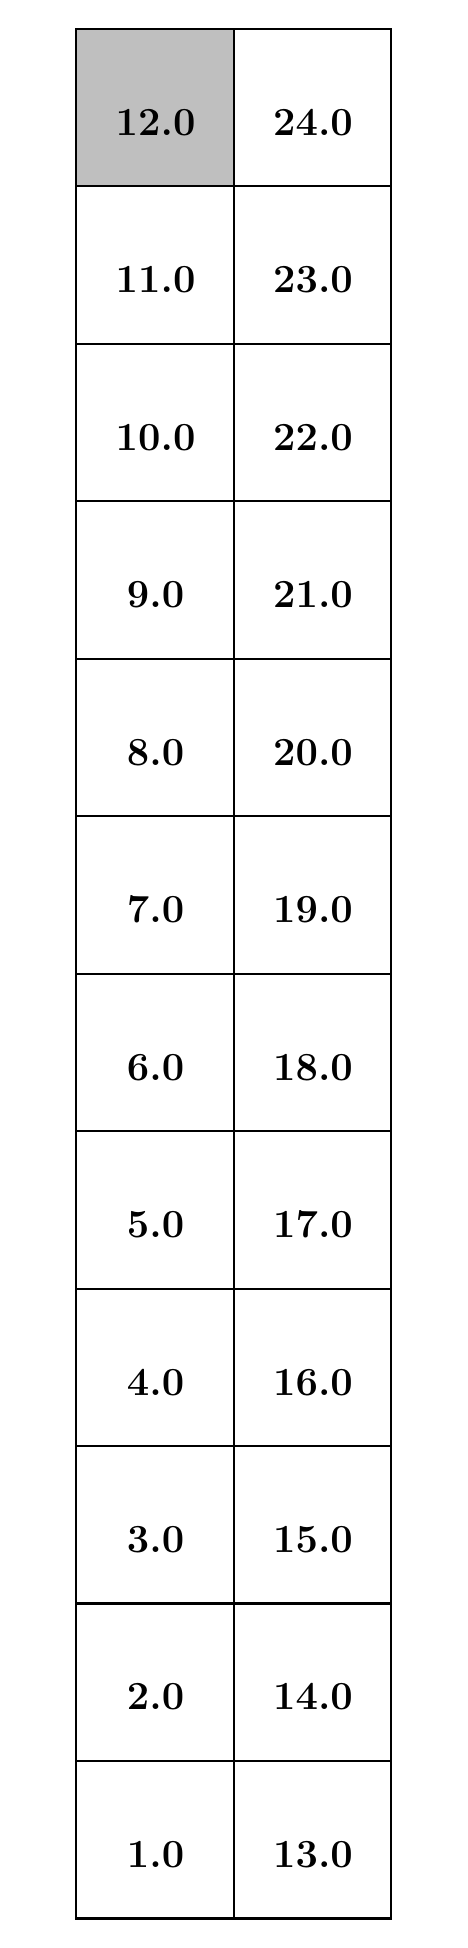
\begin{tikzpicture}
	\draw[black,fill=lightgray] (2,24) rectangle (4,26);
	\foreach \i in {1,...,2} {
		\foreach \j in {1,...,12} {
			\pgfmathsetmacro{\fieldvalue}{\j+12*\i-12}
			\draw[black,thick] (0+2*\i,0+2*\j) rectangle (2+2*\i,2+2*\j);
			\node [text width=3 cm] at (1+2*\i,1+2*\j) {
				\begin{center}
					{\Large \bf \fieldvalue}
				\end{center}
			};
		}
	}
\end{tikzpicture}

\end{center}
\end{document}
